
\minpurp{Netzwerk}
Quelle \textbf{S}, Ziel \textbf{T}

Flusserhaltung: für alle außer Quelle/Ziel: IN = OUT

Totaler Fluss: output(quelle) - input(quelle)


\minmeth{Ford Fulkerson (maximaler Fluss/Schnitt minimaler Kapazität)} Bilde Restgraph aus Netzwerk

\begin{minipage}{0.23\textwidth}
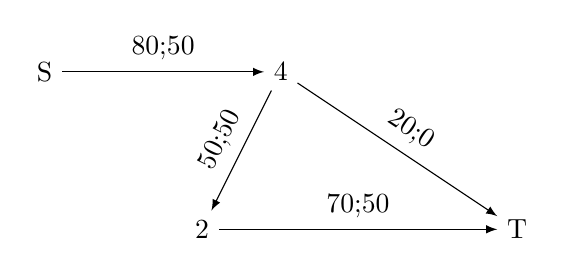
\begin{tikzpicture}[->,>=latex]
\tikzset{EdgeStyle/.append style = {->,bend left =20,black}}
\node(1)  at (0,2) {S}; \node(2) at (2,0){2}; \node(3) at (6,0){T};
\node(4) at (3,2){4};
\draw[->] (2) -> (3) node [above=0.25mm, midway,sloped] {70;50};
\draw[->] (1) -> (4) node [above=0.25mm, midway,sloped] {80;50};
\draw[->] (4) -> (3) node [above=0.25mm, midway,sloped] {20;0};
\draw[->] (4) -> (2) node [above=0.25mm,midway,sloped] {50;50};
\end{tikzpicture}
\end{minipage}$\Rightarrow$
\quarterpage{
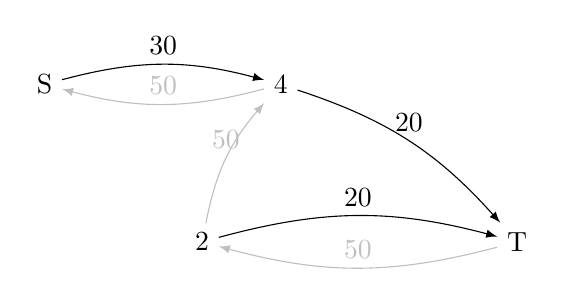
\begin{tikzpicture}[->,>=latex]
\node(1)  at (0,2) {S}; \node(2) at (2,0){2}; \node(3) at (6,0){T};
\node(4) at (3,2){4};
\path (1) edge [above=0.25mm,bend left=15] node  {30} (4);
\path (4) edge [above=0.25mm,bend left=15] node  {20} (3) edge [above=0.25mm,bend left=15,lightgray] node  {50} (1);

\path (2) edge [above=0.25mm,bend left=15, lightgray] node  {50} (4) ;

\path (3) edge [above=0.25mm,bend left=15,lightgray] node  {50} (2);
\path (2) edge [above=0.25mm,bend left=15] node  {20} (3);
\end{tikzpicture}}

Suche Pfad von Quelle -> Ziel, erhöhe fluss an diesem Pfad um dessen minimale Kante\\
Wiederhole solange ein Pfad Quelle -> Ziel existiert

\submeth{Edmonds-Karp} wähle den Pfad im Restgraph mit wenigsten \textbf{Kanten} (durch Weitensuche von der Quelle aus) $\mathbf{O(ke^2)}$\\
\submeth{Schnitt minimaler Kapazität: } Zusammenhangskomponente von S im Restgraph nach Ford-Fulkerson)